\documentclass[letterpaper]{article}

\makeatletter
\newif\ifhtlatex
\@ifpackageloaded{tex4ht}{\htlatextrue}{\htlatexfalse}
\makeatother

\usepackage{amsmath}
\usepackage[margin=0.93in]{geometry}
\usepackage{graphicx}
\usepackage{calc}

\usepackage{hyperref}
\hypersetup{colorlinks=false,pdfborder={0 0 0}}

\def\name{Peter B.~Denton, Ph.D.}
\title{CV}

\pagestyle{myheadings}
\markright{\name}
\thispagestyle{empty}

\usepackage{sectsty}
\sectionfont{\rmfamily\mdseries\Large}
\subsectionfont{\rmfamily\mdseries\itshape\large}
\subsubsectionfont{\rmfamily\mdseries\itshape\normalsize}

\setlength\parindent{0em}

\renewenvironment{itemize}{
\begin{list}{}{
\setlength{\leftmargin}{.5em}}}{
\end{list}}

\begin{document}

\ifhtlatex
\Tag{TITLE+}{CV}
\fi

% % % % % With headshot
% 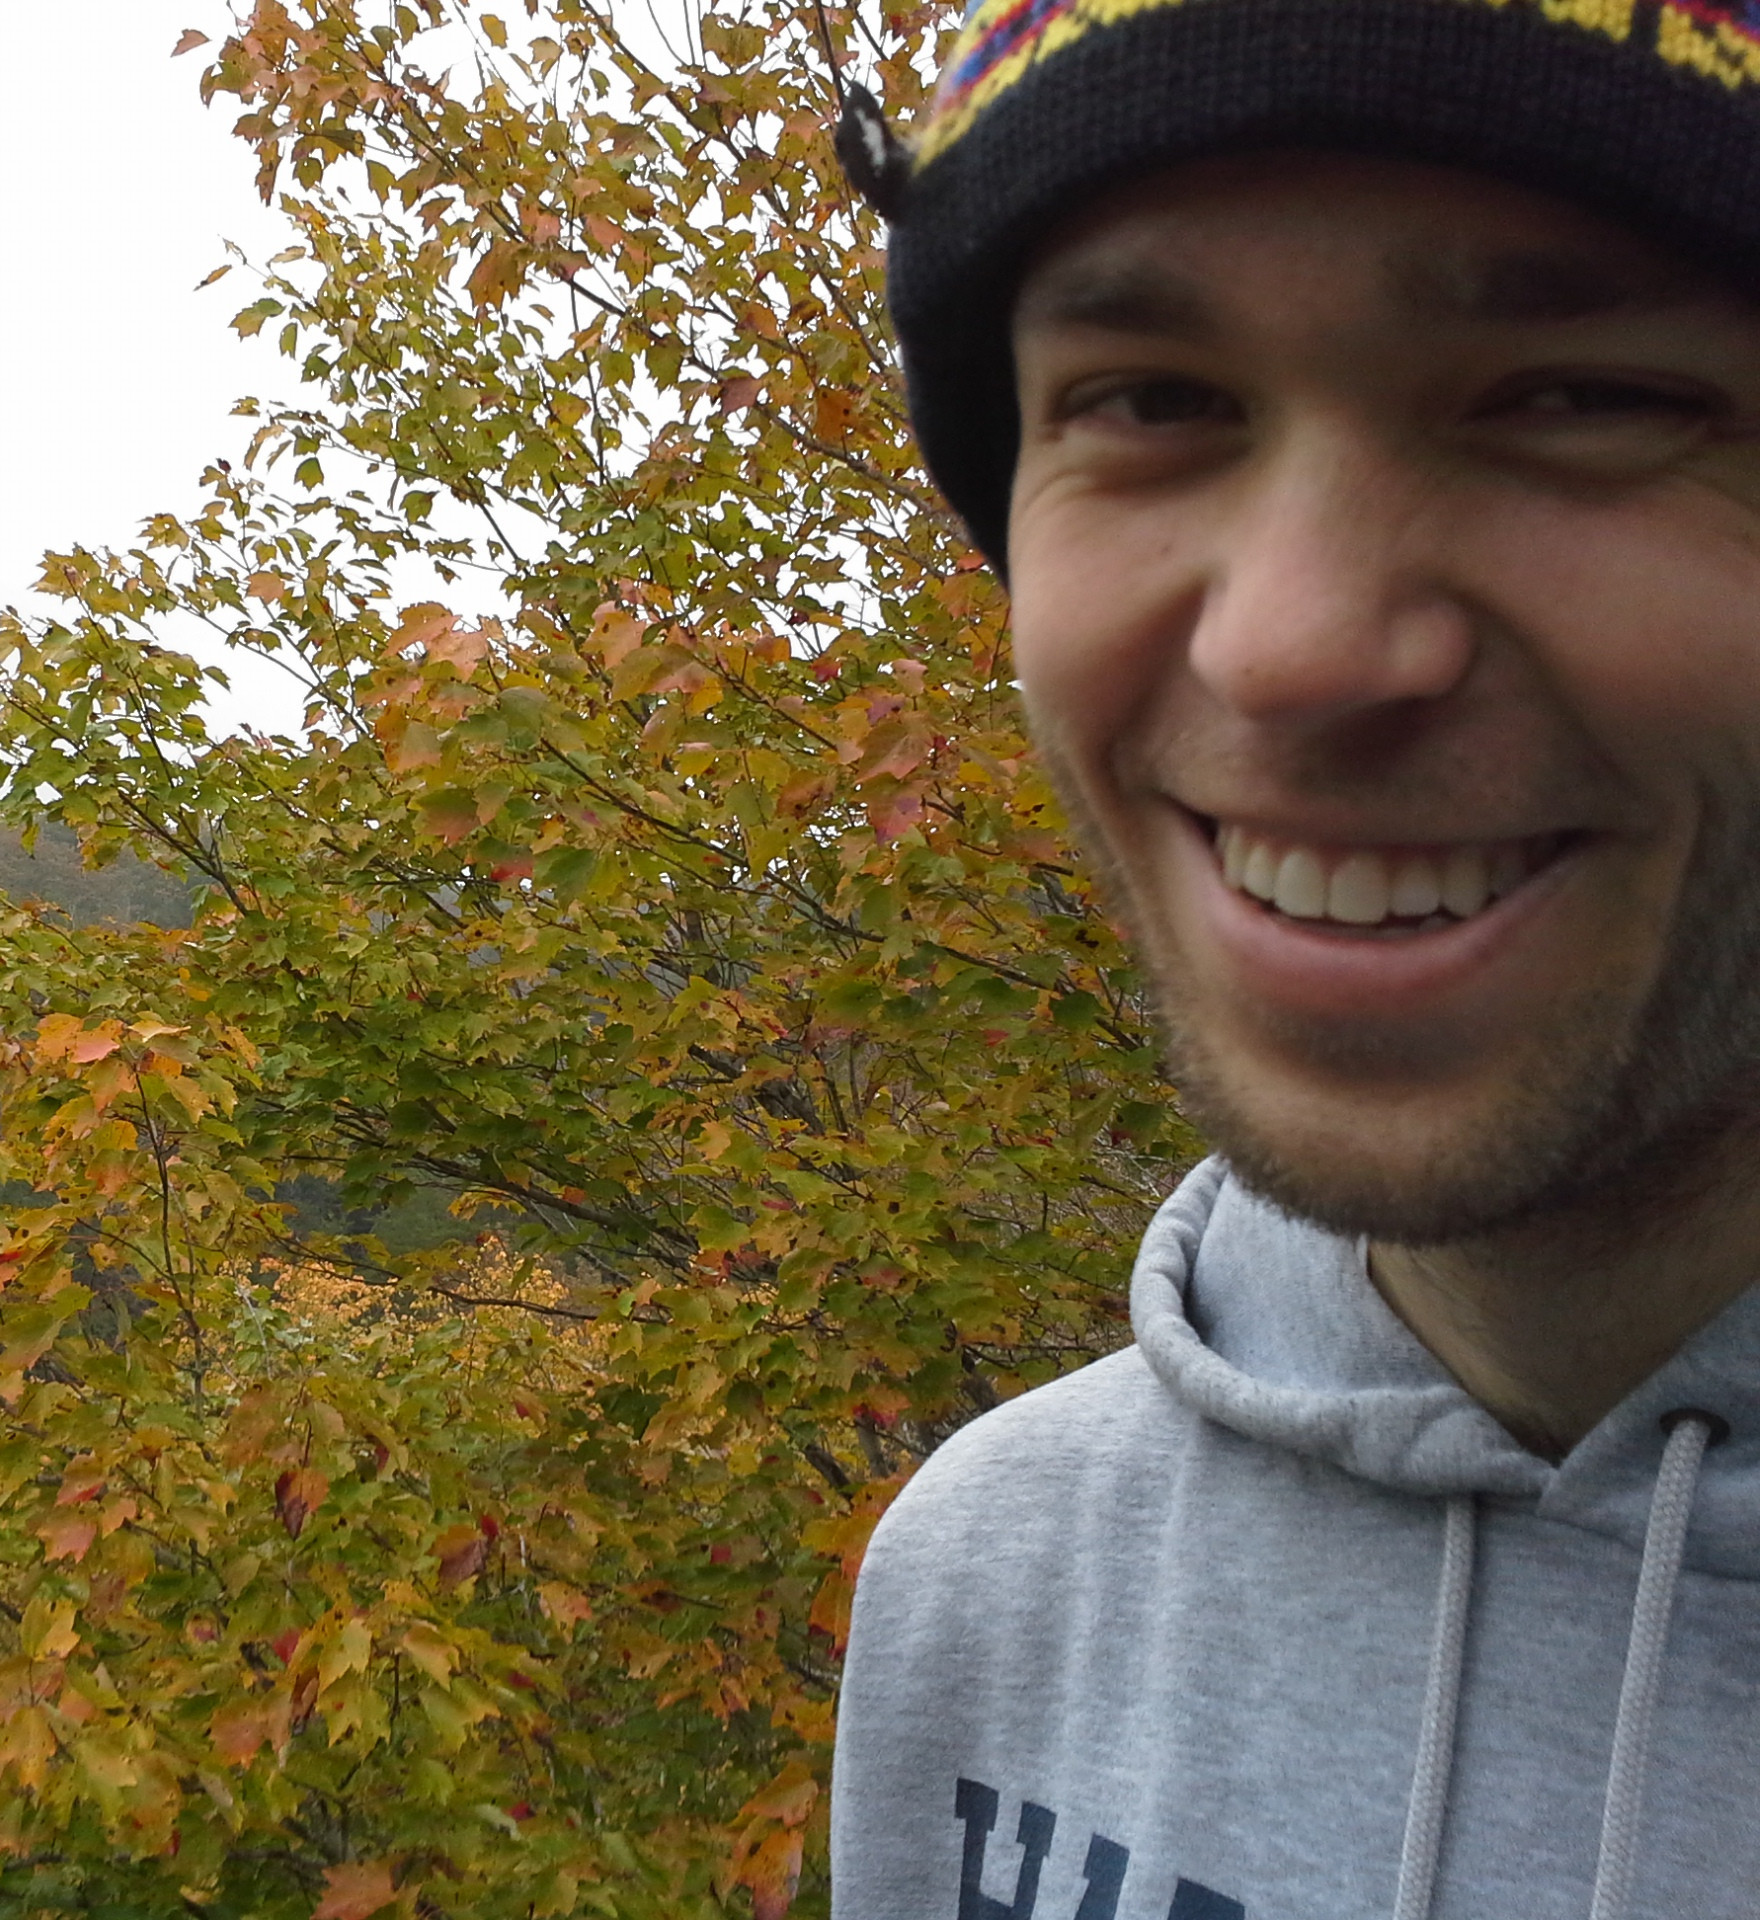
\includegraphics[width=1.2in]{face_cropped}
% \parbox{\textwidth-1.3in}{\vspace*{-1.1in}
% {\huge \name}\\
% \vspace*{0.1in}
% \begin{tabular}{ll|l|ll}
% +45 71 49 29 40 & Gernersgade 35, 1 th & Updated: & \today\\
% \href{mailto:peterbd1@gmail.com}{\tt peterbd1@gmail.com} & Copenhagen K 1319 & Website: & 
% \href{http://peterdenton.github.io}{\tt peterdenton.github.io}
% \end{tabular}
% }

% % % % % Without headshot
{\huge \name}\\
\vspace{0.1in}
\begin{tabular}{ll|l|ll}
Phone: & +45 71 49 29 40 & Gernersgade 35, 1 th & Updated: & \today\\
Email: & \href{mailto:peterbd1@gmail.com}{\tt peterbd1@gmail.com} & Copenhagen K 1319 & Website: & 
\href{http://peterdenton.github.io}{\tt peterdenton.github.io}
\end{tabular}

\subsection*{Research Experience}
\begin{itemize}
\item Postdoctoral Fellow with Irene Tamborra at Niels Bohr International Academy, September 2016--Present.
\item Graduate Student Research Program in Theoretical Physics with Stephen Parke at Fermilab, August 2015--August 2016.
\item DOE funded research assistant with Thomas J.~Weiler at Vanderbilt University, Spring 2011--Fall 2015.
\item Research assistant with Sokrates Pantelides at Vanderbilt University, Summer--Fall 2010.
\item Lee Teng Internship with Tanaji Sen at Fermilab, Summer 2009.
\item Bonner Labs with Bill Llope at Rice University, Summer 2008.
\end{itemize}

\subsection*{Research Interests}
\begin{itemize}
\item SM and BSM neutrino theory.
\item High energy astroparticle physics: neutrinos, UHECRs, anisotropies.
% \item Cosmic ray and neutrino anisotropy searches.
% \item Novel BSM searches at the LHC.
\end{itemize}

\subsection*{Education}
\begin{itemize}
\item Ph.D. Physics, Vanderbilt University, August 2016.
\item B.S. Physics, Rice University, May 2010.
\item B.A. Mathematics, Rice University, May 2010.
% \item Introduction to accelerator physics, United States Particle Accelerator School, 2009.
% \item Multi-variable calculus, differential equations, Grand Rapids Community College, 2005--2006.
\end{itemize}

\subsection*{Physics Schools}
\begin{itemize}
\item Erice International School of Subnuclear Physics in Sicily (ISSP), June 2016.
\item Theoretical Advanced Study Institute in Elementary Particle Physics (TASI), Boulder CO, June 2014.
\end{itemize}

\subsection*{Honors and Awards}
\begin{itemize}
\item The Giorgio Salvini diploma from the Erice International School of Subnuclear Physics, awarded June 2016.
\item PITT PACC travel award of \$300 to attend Pheno '16, awarded April 2016.
\item Vanderbilt Dissertation Enhancement Grant of \$2,000 to attend the Theoretical Advanced Study Institute: Amplitudes For Colliders
in June 2014, awarded April 2014.
\item Subsidy of \$1,600 to attend the Theoretical Advanced Study Institute: Amplitudes For Colliders in June 2014, awarded April 2014.
\item Division of Particles \& Fields travel grant of \$120 to the APS April 2013 meeting, awarded March 2013.
\item The Robert T.~Lagemann Award of \$1,000 for highest academic achievement by a first-year graduate student, awarded April 2011.
\item McMinn Fellowship of \$5,000 a year of five years, awarded March 2010.
\end{itemize}

\subsection*{Language Skills}
\begin{itemize}
\item 
c++, mpi, python, matplotlib, \LaTeX, beamer, ROOT, MATHEMATICA, MATLAB, FORTRAN, gnuplot, java, html, and javascript.
\end{itemize}

\subsection*{Service}
\begin{itemize}
\item Reviewer for Nuclear Physics B.
\item NBIA Astroparticle journal club co-chair, 2017--Present.
\end{itemize}

\subsection*{Students}
\begin{itemize}
\item Klaes M\o ller, University of Copenhagen, master's student, 2017--present.
\item Anna Suliga, University of Copenhagen, master's student, 2017--present.
\item Mia-Louise Nielsen, University of Copenhagen, bachelor's thesis: \emph{The origin of IceCube neutrinos}, 2017.
\end{itemize}

\subsection*{Teaching}
\begin{itemize}
\item Teaching assistant at Vanderbilt University, Fall 2010--Spring 2015.
\item Teaching assistant for the Physics Department at Rice University, Fall 2009.
\item Writing consultant at Rice University, 2007--2010.
\item Tutoring English, math, and physics at middle school, high school, undergraduate, and graduate school levels, 2005--2015.
\end{itemize}

\subsection*{Professional Societies}
\begin{itemize}
\item Member, American Physical Society.
\end{itemize}

\end{document}
